\section{Глубоконеупругое взаимодействие нейтрино с нуклоном}
\subsection{Кинематика и каналы взаимодействия}
Пример глубоконеупругого рассеяния нейтрино  на нуклоне за счет обмена $W$-бозоном, приведен на рис.\ref{fig:DIS}.
\begin{figure}[!h]
\centering
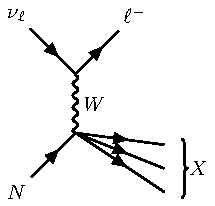
\includegraphics[width=0.4\linewidth]{images/neutrino-nucleon-dis.pdf}
\caption{Диаграмма Фейнмана, соответствующая глубоконеупругому взаимодействию нейтрино с нуклоном через обмен $W$-бозоном.  Существует аналогичная диаграмма с обменом  $Z$-бозоном, при этом $\ell^-\to \nu$.}
\label{fig:DIS}
\end{figure}
Определим кинематические переменные: $k = (E, \bm{k})$ - 4-импульс нейтрино, $k' = (E', \bm{k}')$ 4-импульс  лептона в  конечном состоянии, $p=(M,\bm{0})$ - 4-импульс нуклона, $p'$ - 4-импульс  адронной системы, $q = k-k' = p'-p$. 
Для описания глубоконеупругого события удобно использовать три независимые кинематические переменные: \( Q^2 \), \( x \), \( y \).
Начнём с определения:
\begin{equation}
  Q^2 \equiv -q^2 \approx 2 (EE' - \bm{k} \cdot \bm{k}') \approx 4EE' \sin^2\frac{\theta}{2},
\end{equation}
где \( \theta \) — угол рассеяния лептона в лабораторной системе. В глубоконеупругом рассеянии \( Q^2 > 0 \).

Переменные Бьёркена:
\begin{equation}
  x = \frac{Q^2}{2(p \cdot q)}, \qquad y = \frac{p \cdot q}{p \cdot k}.
\end{equation}
Кроме того, используются: 
\begin{enumerate}
\item $W^2 = (q+p)^2 = M^2+2 (p\cdot q) -Q^2$ - инвариантный квадрат массы адронов,
\item $s = (k+p)^2$ - квадрат энергии в системе центра масс.
\end{enumerate}

% \subsubsection{Партонная модель}
% Чтобы попытаться написать сечение неупругого взаимодействия, нам нужны распределения партонов в самом нуклоне. Обычно их обозначают f(x), подразумевая, что они носят смысл плотности вероятности числа кварков аромата f, имеющих долю импульса в интервале от $x$ до $x+dx$. Тогда $xf(x)$-плотность вероятности доли
% импульса нуклона, переносимая партонами аромата $f$ с долей импульса в интервале от x до $x+dx$. Из изотопической симметрии следуют следующие очевидные равенства:
% \begin{equation}
% \begin{aligned}
%     f_u^p(x) = f_d^n(x) = u(x), &f_d^p(x) = f_u^n(x) = d(x),&f_s^p(x) = f_s^n(x) = s(x) \\
%     f_{\bar{u}}^p(x) = f_{\bar{d}}^n(x) = \bar{u}(x), &f_{\bar{d}}^p(x) = f_{\bar{u}}^n(x) = \bar{d}(x),&f_{\bar{s}}^p(x) = f_{\bar{s}}^n(x) = \bar{s}(x) \\
% \end{aligned}
% \end{equation}
% На рис.(\ref{DIS1}) можно видеть распределения $xf(x)$ взятых из \cite{ParticleDataGroup:2024cfk}.
% \begin{figure}[!h]
% \includegraphics[width=\linewidth]{"images/NuProp/d3"}
% \caption{Плотность вероятности доли
% импульса нуклона, переносимая партонами \cite{ParticleDataGroup:2024cfk}.}
% \label{DIS1}
% \end{figure}
% Cтандартная классификация, связанная с взаимодействием в электрослабой теории, даётся различием между двумя токами:
% \begin{enumerate}
%     \item Если нейтрино взаимодействует с кварком внутри нуклона через $W^{\pm}$-бозон, то продуктами распада будут является лептоны заряженные лептоны и адроны. Такая мода называется заряженым током (СС-ток).
%     \item Если нейтрино взаимодействует с кварком внутри нуклона через $Z$-бозон, то продуктами распада будут является нейтрино и адроны. Такая мода называется нейтральным током (NС-ток).
% \end{enumerate}

%\subsection{Глубоконеупругое рассеяние}

%Дифференциальное сечение глубоко неупругого рассеяния можно записать в виде:
%\begin{equation}
%    \frac{d^2\sigma}{dxdy} = \frac{2\pi y\alpha^2}{Q^4}\sum\limits_j\eta_jL^{\mu\nu}_jH_{\mu\nu}^j,
%\end{equation}
%где сумма берётся по всем возможным промежуточным бозонам, $eta_j$ - множители, зависящие от промежуточного бозона (например, для фотона он равен 1), а лептонный и адронный тензоры даются выражениями:
%\begin{equation}
%\centering
%\begin{aligned}
%    L_{\mu\nu}(k,k') = &2(k_{\mu}k_{\nu}' + k_{\nu}k_{\mu}' - (kk')g_{\mu\nu} - i\epsilon_{\mu\nu\alpha\beta}k^{\alpha}k'^{\beta})\\
%    H_{\mu\nu}(q,P) = &(-g_{\mu\nu} + \frac{q_{\mu}q_{\nu}}{q^2})F_1(x,Q^2) + \frac{P_{\mu}P_{\nu}}{q^2}F_2(x,Q^2)\\
%    &- i\epsilon_{\mu\nu\alpha\beta}\frac{q^{\alpha}P^{\beta}}{2Pq}F_3(x,Q^2),
%\end{aligned}
%\end{equation}
%где $F_i(x,Q^2)$ — это функции, содержащие информацию о структуре неполяризованного адрона. В итоге, переписывая сечения через структурные функции, можно записать выражения для заряженного и нейтрального тока. 
%\begin{equation}
%\centering
%\begin{aligned}
%    \frac{d^2\sigma}{dxdy} = \frac{2\pi y\alpha^2}{Q^4}\eta_i\left((1-y-x^2y^2M^2/Q^2)F_2^i + y^2xF_1^i ± y(1 - 0.5y)xF_3^i\right)
%\end{aligned}
%\end{equation}
%где $i=NC,CC$, а минус и плюс соответствуют нейтрино и антинейтрино в начальном состоянии соответственно.

\subsection{Общий вид сечения}
Сечения нейтрино-нуклонного глубоконеупругого рассеяния вычисляются по следующей универсальной формуле:
\begin{equation}
    \frac{d^2 \sigma^{\text{DIS}}}{dx\,dy} = \frac{G_F^2 M E}{\pi(1 + Q^2/M_W^2)^2} \sum\limits_{i=1}^{5} A_i(x, y, E)\,F_i(x, Q^2),
    \label{eq:xsec_general}
\end{equation}
где $G_F$ — константа Ферми, $M$ — масса нуклона, $E$ — энергия нейтрино, $Q^2$ — переданный импульс, $F_i(x, Q^2)$ — структурные функции, а $A_i(x, y, E)$ — известные кинематические коэффициенты, зависящие от энергии и переменных Бьёркена $x$ и $y$. 

Структурные функции вычисляются на основе партонных распределений, предоставляемых пользователем. Форма коэффициентов $A_i$ зависит от свойств начальных частиц, в частности, от их поляризации. Подробное описание приведено в приложении~\ref{app:structure_functions}.
\section{Взаимодействие нейтрино с электроном}
Так как сечение взаимодействия нейтрино с электроном много меньше нуклонов, то в дальнейшем будет учитываться только резонанс Глешоу ($\bar{\nu}_e+e^{-}\to W^{+}$). Для расчета будем использовать следующие формулы для дифференциальных сечений, взятые из работы~\cite{GANDHI199681}:
\begin{equation}
    \begin{aligned}
\frac{d\sigma(\bar{\nu}_e e \rightarrow \bar{\nu}_e e)}{dy} 
&= \frac{G_F^2 m E_\nu}{2\pi} \left[ \frac{R_e^2}{\left( 1 + 2m E_\nu y / M_Z^2 \right)^2}\right]\\ 
&+ \frac{G_F^2 m E_\nu}{2\pi}\left[\left| \frac{L_e}{1 + 2m E_\nu y / M_Z^2} + \frac{2}{1 - 2m E_\nu / M_W^2 + i F_w / M_w} \right|^2 (1 - y)^2 \right],\\
\frac{d\sigma(\bar{\nu}_e e \rightarrow \bar{\nu}_\mu \mu)}{dy} 
&= \frac{G_F^2 m E_\nu}{2\pi} \frac{4(1-y)^2 [1-(\mu^2-m^2)/2mE_\nu]^2}{(1-2mE_\nu/M_W^2)^2 + \Gamma_W^2/M_W^2}, \\
\frac{d\sigma(\bar{\nu}_e e \rightarrow \text{hadrons})}{dy} 
&= \frac{d\sigma(\bar{\nu}_e e \rightarrow \bar{\nu}_\mu \mu)}{dy} \frac{\Gamma(W \rightarrow \text{hadrons})}{\Gamma(W \rightarrow \mu \bar{\nu}_\mu)},
\end{aligned}
\end{equation}
